
Exploration strategies balance the sensitive exploration and exploitation trade-off. Exploration is needed, especially in the early stages of learning a new part of the episode, to allow the agent to uncover new experiences which maximum the Q-value. Meanwhile, exploitation is also needed to force the agent to converge through taking the path with the maximum Q-value at that point.

Exploration strategies can be divided into two use cases: discrete spaces, $\epsilon$-greedy (\cite{sutton1998reinforcement}) and Boltzmann, and continuous spaces. For rocket landing, the state space (e.g., position, velocity, orientation) and the action space (e.g., thrust levels, gimbal angles) are continuous; as such only these strategies continuous strategies are covered.

\textbf{Action noise-based exploration} is an efficient way to encourage exploration in continuous space by adding noise.
\begin{itemize}
    \item \textit{Gaussian Noise}: in \cite{lillicrap2015continuous}, the exploration policy is created by adding random noise to the actor's policy. This is used in several actor-critic RL configurations used for learning on a continuous domain, like the Twin Delayed Deep Deterministic Policy Gradient (TD3) algorithm wrote in \autoref{sec:TD3}.

    \item \textit{Ornstein-Uhlenbeck (OU) noise}: is used to temporary correlate noise, \cite{lillicrap2015continuous} use this to enhance their exploration efficiency, showing it is good for "physical control problems with inertia".

    \item \textit{Adaptive Noise Scaling}: can be combined with a method above to balance exploration-exploitation during training. Here the noise is scaled is automatically altered, like in soft actor critic (SAC) shown in \autoref{sec:SAC}
\end{itemize}

\begin{tcolorbox}[title={\textbf{Lemma. Gaussian and OU noise}}]
Exploration in deterministic reinforcement learning methods like DDPG, D4PG or TD3 explained later in \autoref{sec:off_policy} requires the injection of external noise into the policy's action space to discover new and unseen solutions.  Two common types of noise processes are Gaussian and OU noise.

\textbf{Gaussian noise} is temporally uncorrelated and drawn independently at each timestep from a normal distribution. This noise is simple and suitable for environments where smoothness in action evolution over time is not critical.
\[
    \epsilon_t \sim \mathcal{N}(0, \sigma^2)
\]


\textbf{Ornstein–Uhlenbeck noise} introduces temporal correlation by modelling the stochasticity as mean-reverting process, meaning that the stochastic process tends to revert towards a long term mean. This mean-reverting proces temporally smooths noise, idea for physical control tasks with momentum like rocket landing where a sudden change in action can lead to instability. The correlation across timesteps simulates inertia, yielding more natural and consistent exploration trajectories.

\[
    \epsilon_{t+1} = \epsilon_t + \theta (\mu - \epsilon_t) \Delta t + \sigma \sqrt{\Delta t} \mathcal{N}(0, 1)
\]

Gaussian noise is simpler to implement than OU noise, however OU noise encourages smoother transitions in systems with momentum, like physical control tasks.
\end{tcolorbox}


\textbf{Parameter Space Noise} (PSN) was introduced to overcome the downfall of the action space noise of inconsistent exploratory behaviours due to a fixed state always giving different actions. This can give problems like early truncation where at points in the episode the action is sensitive to noise and needs to be precise. However, adaptive noise scaling to push the action space noise to small amounts at parts in the episode can overcome this problem. PSN adds noise through \autoref{eq:PSM} to perturb the policy network parameters at the start of each episode and maintain them fixed afterwards; this results in state-dependent actions, unlike Gaussian noise methods.

\begin{equation}
    \tilde{\theta} = \theta + \mathcal{N}(0, \sigma^2 \cdot I)
\label{eq:PSM}
\end{equation}

PSN has been experimented with in \cite{plappert2018parameter}, building on the work of \cite{sehnke2010parameter} and \cite{rucksties2008state}; they show PSN offers better exploration and avoids suboptimal converge on continuous environments, and has significant benefits in environments with sparse rewards, along with outperforming Evolutionary Strategies (ES).


In environments where extrinsic rewards are sparse, intrinsic rewards can allow the agent to explore better; this can be employed through an \textbf{Intrinsic Curiosity Module} (ICM) developed in \cite{pathak2017curiosity}, which encourages the agent to explore. Intrinsic rewards are provided by the agent's own experience, motivating them to explore without extrinsic rewards.

An inverse model, which predicts the action \(\hat{a}(s_t, s_{t+1})\), is trained via \autoref{eq:loss_ICM_inverse} to minimise the loss between the actual and predicted actions. The forward model predicts the next state's features \(\hat{\phi}_{s_{t+1}}(\phi_{s_t}, a_t)\), through minimisation in state feature prediction via \autoref{eq:loss_ICM_forward}. The intrinsic reward, \autoref{eq:intrinisic_reward}, depends on the hyperparameter $\eta$ acting as the scaling factor. The total resulting reward is the sum of the extrinsic and intrinsic rewards.

\begin{equation}
    L_I(\hat{a}_t, a_t; \theta^I) = -\log P(a_t | s_t, s_{t+1}; \theta^I)
\label{eq:loss_ICM_inverse}
\end{equation}

\begin{equation}
    L_F(\phi(s_t), \hat{\phi}(s_{t+1}; \theta^F)) = \frac{1}{2} \|\phi(s_{t+1}) - \hat{\phi}(s_{t+1}; \theta^F)\|^2
\label{eq:loss_ICM_forward}
\end{equation}

\begin{equation}
    R^{\text{intrinsic}}_t = \eta \cdot \frac{1}{2} \|\phi(s_{t+1}) - \hat{\phi}(s_{t+1}; \theta^F)\|^2
\label{eq:intrinisic_reward}
\end{equation}

An alternative to ICM is \textbf{Random Network Distillation} (RND), introduced in \cite{burda2018exploration}, where they argue it is simpler and more stable than ICM, through testing on Montezuma's Revenge. This method works well for sparse reward environments, allowing extrinsic and intrinsic rewards to be flexibly combined. Here, intrinsic rewards are based upon a prediction error from a trainable "prediction" network approximating a fixed and randomly initialised "target" network. The prediction network is trained to minimise the prediction error through \autoref{eq:RND_1}. The intrinsic reward can be set equal to the prediction network loss, as such states explored less will gain a higher prediction error, and thus, the RND encourages them to be explored; this process is visualised in \autoref{fig:RND}. In essence, RND measures how novel a state is by comparing prediction error on a fixed random target network.

\begin{equation}
    L_{\text{predict}} = \frac{1}{2} \cdot ||y_{\text{target}} - y_{\text{predict}} ||^2 = r_{\text{intrinsic}}
\label{eq:RND_1}
\end{equation}

\begin{figure}[H]
    \centering
    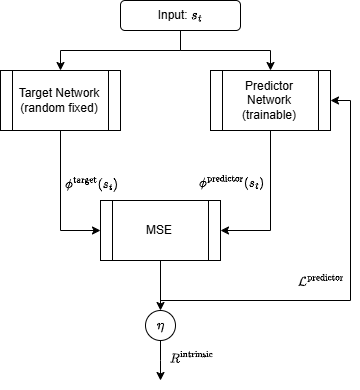
\includegraphics[width=0.5\linewidth]{figures/LiteratureStudy/RL_diagram_RND.png}
    \caption{Flow diagram showing how RND works.}
    \label{fig:RND}
\end{figure}

\textbf{Noisy networks} (\cite{fortunato2017noisy}) incorporate parametric noise into the network weights to enhance exploration efficiency via stochastic diversity of the agent's policy. Here, Stochastic Gradient Descent (SGD) learns the noise scale, adapting it over time; for instance, less noise is present as the agent becomes more confident, decreasing exploration. The authors also show how it is compatible with any RL architecture which employs SGD. Ultimately arguing, noisy networks provide structured and adaptive exploration.